% Drawing 154/07-9 -- folder 154, batch 07, archive page 132 (PDF page 133).
% Transcription: en haut à gauche, un dessin en couleur : un fuseau (bigone) bordé d'un arc vert foncé et d'un arc vert clair, entre deux croisements orange, traversé de pseudo-droites orange et de cinq courbes brunes numérotées $1$ à $5$ aux deux bouts, qui le balaient ; au milieu, un second dessin du même fuseau, les courbes numérotées $1$ à $8$, les croisements marqués « $1 = 5$ », « $2$ », « $3$ », « $4$ », « $5 = 8$ » (en orange), « $5/6$ » sur l'arc supérieur et « $1/2$ » sur l'inférieur
% Kind: spindles between two crossings swept by numbered brown curves; small crossing; circle with D_0 ... D_nu. Method 2 (schematic redraw from the facsimile). Status: partial.
% Notes: Top left, a colour drawing: a spindle (bigon) bordered by a dark green (blue-green) arc and a light green arc, between two orange crossings, crossed by orange pseudolines and by five brown curves numbered 1 to 5 at both ends, which sweep it. In the middle, a larger version of the same, the curves numbered 1 to 5 on the left and up to 8 on the right. To the right, a small crossing on a light green line with s, p, D; below in the middle, a pencil circle with spokes labelled D_0, D_1, ... (labels not reproduced). Curves schematic; read from the page view.
% Coordinates: 1 unit = 1 mm = 1/100 of the crop width (bbox in page fractions: [0.175, 0.111, 0.837, 0.4]).
% Redrawn by Claude (claude-opus-5-5), issue #73, 2026-11-07; not checked by a human; not compiled (no TeX in the session).
% Rights: reproduces part of the work -- behind RENDER_TRANSCRIPTS, never published by itself.
\documentclass[tikz,border=3pt]{standalone}
\usepackage{amsmath,amssymb}
\usetikzlibrary{patterns,arrows.meta}
\tikzset{Or/.style={orange!90!black}, Ye/.style={yellow!80!orange}, Lg/.style={green!60!black!70}, Dg/.style={green!45!black}, Br/.style={brown!80!black}, Rd/.style={red!85!black}, Bl/.style={blue!70!black}, Gy/.style={black!40}, pencil/.style={black!45}, struck/.style={black!35}, mark/.style={circle,draw,inner sep=1.3pt}, pt/.style={circle,fill,inner sep=0.9pt}, opt/.style={circle,draw,fill=white,inner sep=1.1pt}}
\begin{document}
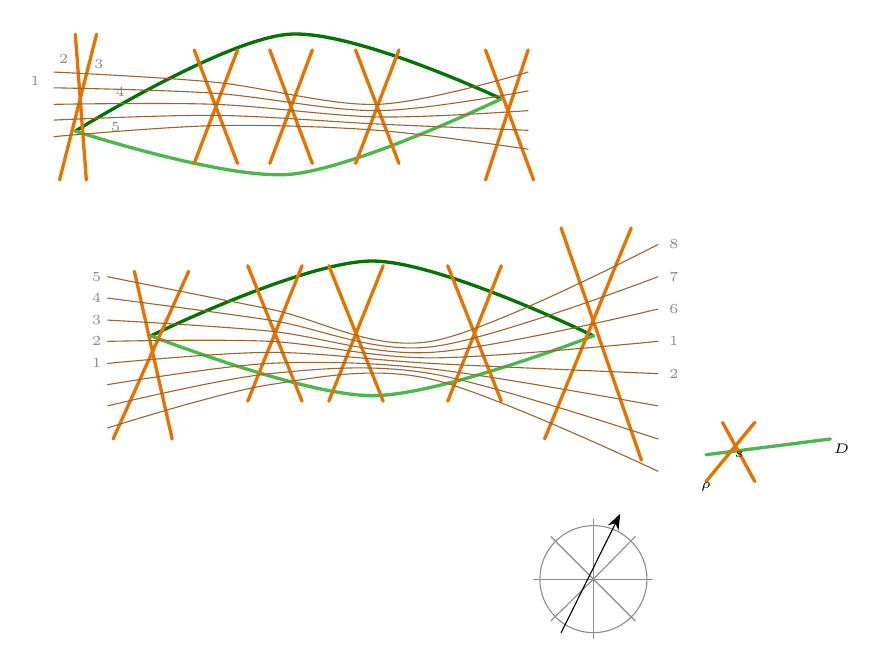
\begin{tikzpicture}[x=1mm,y=1mm,line cap=round,line join=round,font=\scriptsize]
\draw[Dg,very thick] plot[smooth, tension=0.55] coordinates {(4.1,-13) (31.2,-0.7) (58.2,-8.9)};
\draw[Lg,very thick] plot[smooth, tension=0.55] coordinates {(4.1,-13) (31.2,-18.5) (58.2,-8.9)};
\draw[Or,very thick] (2.1,-19.2) -- (6.8,-0.7);
\draw[Or,very thick] (4.1,-0.7) -- (5.5,-19.2);
\draw[Or,very thick] (19.2,-2.7) -- (24.7,-17.1);
\draw[Or,very thick] (24.7,-2.7) -- (19.2,-17.1);
\draw[Or,very thick] (28.8,-2.7) -- (34.2,-17.1);
\draw[Or,very thick] (34.2,-2.7) -- (28.8,-17.1);
\draw[Or,very thick] (39.7,-2.7) -- (45.2,-17.1);
\draw[Or,very thick] (45.2,-2.7) -- (39.7,-17.1);
\draw[Or,very thick] (56.2,-2.7) -- (62.3,-19.2);
\draw[Or,very thick] (61.6,-2.7) -- (56.2,-19.2);
\draw[Br] plot[smooth, tension=0.55] coordinates {(1.4,-5.5) (21.9,-6.8) (42.5,-9.6) (61.6,-5.5)};
\draw[Br] plot[smooth, tension=0.55] coordinates {(1.4,-7.5) (21.9,-8.2) (42.5,-10.4) (61.6,-7.9)};
\draw[Br] plot[smooth, tension=0.55] coordinates {(1.4,-9.6) (21.9,-9.6) (42.5,-11.2) (61.6,-10.4)};
\draw[Br] plot[smooth, tension=0.55] coordinates {(1.4,-11.6) (21.9,-11) (42.5,-12.1) (61.6,-12.9)};
\draw[Br] plot[smooth, tension=0.55] coordinates {(1.4,-13.7) (21.9,-12.3) (42.5,-12.9) (61.6,-15.3)};
\node[inner sep=1pt,pencil] at (-1,-6.6) {\tiny 1};
\node[inner sep=1pt,pencil] at (2.6,-3.9) {\tiny 2};
\node[inner sep=1pt,pencil] at (7.1,-4.5) {\tiny 3};
\node[inner sep=1pt,pencil] at (9.8,-8.1) {\tiny 4};
\node[inner sep=1pt,pencil] at (9.2,-12.5) {\tiny 5};
\draw[Dg,very thick] plot[smooth, tension=0.55] coordinates {(13.7,-39) (41.8,-29.5) (69.9,-39)};
\draw[Lg,very thick] plot[smooth, tension=0.55] coordinates {(13.7,-39) (41.8,-46.6) (69.9,-39)};
\draw[Or,very thick] (8.9,-52.1) -- (18.5,-30.8);
\draw[Or,very thick] (11.6,-30.8) -- (16.4,-52.1);
\draw[Or,very thick] (26,-30.1) -- (32.9,-47.3);
\draw[Or,very thick] (32.9,-30.1) -- (26,-47.3);
\draw[Or,very thick] (36.3,-30.1) -- (43.2,-47.3);
\draw[Or,very thick] (43.2,-30.1) -- (36.3,-47.3);
\draw[Or,very thick] (51.4,-30.1) -- (58.2,-47.3);
\draw[Or,very thick] (58.2,-30.1) -- (51.4,-47.3);
\draw[Or,very thick] (65.8,-25.3) -- (76,-54.8);
\draw[Or,very thick] (74.7,-25.3) -- (63.7,-52.1);
\draw[Br] plot[smooth, tension=0.55] coordinates {(8.2,-31.5) (28.8,-35.6) (49.3,-39.7) (78.1,-27.4)};
\draw[Br] plot[smooth, tension=0.55] coordinates {(8.2,-34.2) (28.8,-37) (49.3,-40.4) (78.1,-31.5)};
\draw[Br] plot[smooth, tension=0.55] coordinates {(8.2,-37) (28.8,-38.4) (49.3,-41.1) (78.1,-35.6)};
\draw[Br] plot[smooth, tension=0.55] coordinates {(8.2,-39.7) (28.8,-39.7) (49.3,-41.8) (78.1,-39.7)};
\draw[Br] plot[smooth, tension=0.55] coordinates {(8.2,-42.5) (28.8,-41.1) (49.3,-42.5) (78.1,-43.8)};
\draw[Br] plot[smooth, tension=0.55] coordinates {(8.2,-45.2) (28.8,-42.5) (49.3,-43.2) (78.1,-47.9)};
\draw[Br] plot[smooth, tension=0.55] coordinates {(8.2,-47.9) (28.8,-43.8) (49.3,-43.8) (78.1,-52.1)};
\draw[Br] plot[smooth, tension=0.55] coordinates {(8.2,-50.7) (28.8,-45.2) (49.3,-44.5) (78.1,-56.2)};
\node[inner sep=1pt,pencil] at (6.8,-31.5) {\tiny 5};
\node[inner sep=1pt,pencil] at (6.8,-34.2) {\tiny 4};
\node[inner sep=1pt,pencil] at (6.8,-37) {\tiny 3};
\node[inner sep=1pt,pencil] at (6.8,-39.7) {\tiny 2};
\node[inner sep=1pt,pencil] at (6.8,-42.5) {\tiny 1};
\node[inner sep=1pt,pencil] at (80.1,-27.4) {\tiny 8};
\node[inner sep=1pt,pencil] at (80.1,-31.5) {\tiny 7};
\node[inner sep=1pt,pencil] at (80.1,-35.6) {\tiny 6};
\node[inner sep=1pt,pencil] at (80.1,-39.7) {\tiny 1};
\node[inner sep=1pt,pencil] at (80.1,-43.8) {\tiny 2};
\draw[Lg,very thick] (84.2,-54.1) -- (100,-52.1);
\draw[Or,very thick] (84.2,-57.5) -- (90.4,-50);
\draw[Or,very thick] (86.3,-50) -- (90.4,-57.5);
\node[inner sep=1pt] at (88.4,-54.1) {\tiny $s$};
\node[inner sep=1pt] at (84.2,-58.2) {\tiny $\rho$};
\node[inner sep=1pt] at (101.4,-53.4) {\tiny $D$};
\draw[pencil] (69.9,-69.9) circle[radius=6.8];
\draw[pencil] (69.9,-69.9) -- (77.4,-69.9);
\draw[pencil] (69.9,-69.9) -- (75.2,-64.5);
\draw[pencil] (69.9,-69.9) -- (69.9,-62.3);
\draw[pencil] (69.9,-69.9) -- (64.5,-64.5);
\draw[pencil] (69.9,-69.9) -- (62.3,-69.9);
\draw[pencil] (69.9,-69.9) -- (64.5,-75.2);
\draw[pencil] (69.9,-69.9) -- (69.9,-77.4);
\draw[pencil] (69.9,-69.9) -- (75.2,-75.2);
\draw[-{Stealth[length=2mm]}] (65.8,-76.7) -- (73.3,-61.6);
\end{tikzpicture}
\end{document}
